\newcommand{\DSAToPAT}{DSA$\to$PAT\xspace}
\newcommand{\Code}[1]{\texttt{#1}}

\chapter{Search for Displaced Dimuons in CMS at 13~TeV}

\section{Trigger, Data, and Simulation}
\subsection{Trigger}
\label{sec:dd:trigger}
As mentioned in \Sec~\ref{cms:trigger}, defining criteria on which to trigger is the first stage of an analysis.
Typical CMS analyses using muons search for new particles produced in the hard interactions of \pp collisions that decay quickly into muons.
Such muons appear to originate directly from the point of interaction of the crossing beams, or beamspot.
For this reason, the reconstruction of muon tracks used by most trigger paths includes the beamspot, referred to as a beamspot constraint.
But muons produced from the decay of a long-lived particle may very well not point towards the beamspot.
Therefore, dedicated triggers without beamspot constraints are necessary to collect data containing long-lived particles.

The HLT path that collected the 2016 data studied in this analysis was
$$\Code{HLT\_L2DoubleMu28\_NoVertex\_2Cha\_Angle2p5\_Mass10}$$
The abbreviations in this expression define the various criteria:
\begin{itemize}
  \item \texttt{\textbf{L2DoubleMu28}}: requirement that two muons be reconstructed using only the muon system, each with a $\pT$ of at least 28\GeV. The muon system requirement is the first step towards ensuring that the triggered objects are really muons, as well as allowing the analysis to be sensitive to a range of possible lifetimes. The \pT requirement keeps the rate of triggered events in the data acquisition system within its maximum rate and allows the analysis to focus on events in a regime with reduced contributions from complex QCD processes.
  \item \texttt{\textbf{NoVertex}}: requirement that no beamspot constraint be imposed in the muon reconstruction. As mentioned above, this requirement is intended to improve the reconstruction of muons originating from a displaced vertex that do not point towards the beamspot.
  \item \texttt{\textbf{2Cha}}: requirement that muon segments be present in at least two CSC or DT stations. This requirement selects muons with hits over multiple chambers, which is necessary to reconstruct them with high quality.
  \item \texttt{\textbf{Angle2p5}}: requirement that the 3D angle between the muons $\alpha$ be at least 2.5\unit{rad} (equivalent to $\cos{\alpha} > -0.8$). This requirement is intended to prevent cosmic ray muons from passing the trigger, as the reconstruction algorithms usually reconstruct cosmic ray muons as a pair of back-to-back muons, \ie $\alpha \sim \pi$ or $\cos(\alpha) \sim -1$.
  \item \texttt{\textbf{Mass10}}: requirement that the invariant mass of the two muon system $M_{\mu\mu}$ be at least 10\GeV. As with the \pT requirement above, this requirement also serves to keep the event rate within acceptable thresholds and reduce consideration of events dominated by complex QCD processes.
\end{itemize}

$$\text{PLOT OF TRIGGER EFFICIENCY}$$

\subsection{Data Samples}
The analysis uses data taken from \pp collisions at the LHC center-of-mass energy of 13\TeV during the data taking period of 2016, corresponding to an integrated luminosity of 35.9\fbinv.
The CMS datasets used are reprocessed under the CMS software version \Code{CMSSW\_8\_0\_31} in August 2017, known as the ``re-reco'' data.
This analysis consequently uses the same CMS software version for all its analysis.
CMS data are organized into runs consisting of individual lumi sections, which are time intervals of data taking at CMS corresponding to approximately 23\unit{s}.
A dedicated data quality management team certifies CMS data by producing lists of run numbers approved for physics analysis.
\Tab~\ref{tab:dd:data} lists the names of the datasets used in this analysis, their certified run range, and their corresponding integrated luminosity for each of the data taking eras of 2016.

\begin{table}
  \centering
  \begin{tabular}{lcr}
    \hline
    Dataset & Run Range & \multicolumn{1}{c}{\intlumi} \\
    \hline
    \Code{DoubleMuon/Run2016B-07Aug17\_ver2-v1/AOD} & 273150--275376 &          5.75\fbinv  \\
    \Code{DoubleMuon/Run2016C-07Aug17-v1/AOD}       & 275656--276283 &          2.57\fbinv  \\
    \Code{DoubleMuon/Run2016D-07Aug17-v1/AOD}       & 276315--276811 &          4.24\fbinv  \\
    \Code{DoubleMuon/Run2016E-07Aug17-v1/AOD}       & 276831--277420 &          4.02\fbinv  \\
    \Code{DoubleMuon/Run2016F-07Aug17-v1/AOD}       & 277932--278808 &          3.10\fbinv  \\
    \Code{DoubleMuon/Run2016G-07Aug17-v1/AOD}       & 278820--280385 &          7.58\fbinv  \\
    \Code{DoubleMuon/Run2016H-07Aug17-v1/AOD}       & 281613--284044 &          8.65\fbinv  \\
    \hline
    \textbf{Total}                                  &                & \textbf{35.92\fbinv} \\
    \hline
  \end{tabular}
  \caption{CMS datasets used by the analysis, including dataset names, the ``Golden'' run ranges as certified by CMS for physics analysis, and integrated luminosities, taken from Reference~\cite{PdmV2016} and following embedded links. Integrated luminosity values were obtained from running the standard \Code{brilcalc} prescription found at Reference~\cite{BrilcalcQuickStart}.}
  \label{tab:dd:data}
\end{table}

\subsection{Monte Carlo Simulation Samples of Signal and Background}
Comparing theoretical predictions to CMS data is a complex task which must connect scattering amplitudes of the hard process underlying the \pp collision computed via perturbative methods in quantum field theory to the production of particles and their passage through the material of CMS to the response and subsequent data obtained by the CMS detectors.
Numerical simulation is used to obtain these predictions, and because Monte Carlo methods are used to model stochastic effects at each stage, this simulation is described as Monte Carlo (MC) simulation.
This analysis uses simulation of signal models as well as simulation of background processes in its studies.

\Tab~\ref{tab:dd:signalsamples} lists the MC simulation samples of the BSM Higgs $\PHiggs \to \PLLP\PLLP$ benchmark signal model described in Chapter~\ref{chap:theory}.
Both 4$\mu$ final states, in which both long-lived particles decay to two muons, and 2$\mu$ final states, in which one long-lived particle decays to two muons and the other does not, are simulated.
Samples were produced for several combinations of BSM Higgs masses (\mH), long-lived particle masses (\mX), and long-lived particle lifetimes (\cTau).
The lifetimes were chosen such that the mean decay lengths in the transverse plane are 3\cm, 30\cm, and 250\cm in the laboratory frame.

\begin{table}
  \centering
  \begin{tabular}{ccccc}
    \hline
    \mH (\GeV) & \mX (\GeV) & \multicolumn{3}{c}{\cTau (\mm)} \\
    \hline
    \multirow{4}{*}{1000} & 350 & 35 & 350 & 3500 \\
                          & 150 & 10 & 100 & 1000 \\
                          &  50 &  4 &  40 &  400 \\
                          &  20 &  2 &  20 &  200 \\
    \hline
    \multirow{3}{*}{400}  & 150 & 40 & 400 & 4000 \\
                          &  50 &  8 &  80 &  800 \\
                          &  20 &  4 &  40 &  400 \\
    \hline
    \multirow{2}{*}{200}  &  50 & 20 & 200 & 2000 \\
                          &  20 &  7 &  70 & 7000 \\
    \hline
    \multirow{2}{*}{125}  &  50 & 50 & 500 & 5000 \\
                          &  20 & 13 & 130 & 1300 \\
    \hline
  \end{tabular}
  \caption{Simulated $\PHiggs \to \PLLP\PLLP$ signal samples used by the analysis, for several combinations of BSM Higgs mass (\mH), long-lived particle mass (\mX), and long-lived particle lifetime (\cTau).}
  \label{tab:dd:signalsamples}
\end{table}

The main backgrounds for this analysis are
\begin{itemize}
  \item the Drell-Yan process yielding dileptons (Z/$\gamma^* \to \ell\ell$), especially from reconstruction mistakes;
  \item QCD processes yielding dileptons, especially from cascade decays of bottom quarks and hadron decays in flight; and
  \item cosmic ray muons reconstructed as dileptons
\end{itemize}
Other backgrounds from top quark production and diboson production with leptonic decays produce negligible contributions.
The CMS collaboration centrally produces MC simulation of background processes for physics analysis; this analysis uses the ``Summer16'' campaign produced for Moriond~2017.
\Tab~\ref{tab:dd:bgsamples} lists the MC simulation samples of background processes used in this analysis, with the total production cross section and the number of generated events, and an ``equivalent luminosity'' defined in the next section that is important for understanding the statistical power of the simulation.
These MC background samples are useful for many studies, but have some important limitations:
\begin{itemize}
  \item The Drell-Yan and QCD processes are the dominant sources of background events in \pp collisions and are simulated. However, the reconstruction mistakes producing this background may not be well modeled, and the simulation of QCD events is known to not accurately reproduce data.
  \item The Drell-Yan and QCD samples also have limited statistical power, as the number of generated events is fewer than the number of expected events in 2016 data.
  \item The available MC simulation of cosmic muons does not include simulation of showers of cosmic muons nor of cosmic muons mixed with \pp collisions.
\end{itemize}
For these reasons, MC simulation of background does not provide a good description of the expected background, so optimization of the analysis as well as evaluation of the expected background is consequently performed using data.
MC simulation of background is therefore primarily used to study general trends and gain insights.

\begin{table}
  \centering
  \begin{tabular}{llD{.}{.}{6.3}rD{.}{.}{3.2}}
    \hline
    Process & Kinematic Cuts & \multicolumn{1}{c}{$\sigma$ (\unit{pb})} & Events & \multicolumn{1}{c}{$\intlumi^\text{eq}$ (\fbinv)} \\
    \hline
    Z/$\gamma^* \to \ell\ell$          & $10\GeV < M_{\ell\ell} < 50\GeV$ &  18810     &   30,935,823 &   1.20\\
    Z/$\gamma^* \to \ell\ell$          & $M_{\ell\ell} > 50\GeV$          &   6225     &  122,547,040 &  13.19\\
    QCD $\mu$-enriched                 & $\pT > 20\GeV$                   & 302672.16  &   22,094,081 &   0.07\\
    $t\overline{t} \to \ell\ell\nu\nu$ &                                  &     87.31  &   79,140,880 & 906.44\\
    $t$W, $\overline{t}$W              &                                  &     35.8   &   13,885,924 & 387.87\\
    WZ                                 &                                  &     47.13  &    6,995,142 &  84.82\\
    ZZ                                 &                                  &     16.523 &    2,986,132 & 120.32\\
    WW $\to \ell\ell\nu\nu$            &                                  &     12.178 &    1,999,000 & 164.15\\
    W+jets                             &                                  &  61526.7   &   29,804,825 &   0.48\\
    \hline
  \end{tabular}
  \caption{CMS simulation samples used by the analysis for each background process, along with the total production cross section and the number of generated events. Simulated events are scaled to correspond to the total integrated luminosity in 2016 (35.9\fbinv) by scaling proportionally to the equivalent luminosity in 2016, $\intlumi^\text{eq}$, given in the table.}
  \label{tab:dd:bgsamples}
\end{table}

Simulation of the hard process including matrix element computation is performed by \POWHEG in all signal and background samples, except for the Drell-Yan (Z/$\gamma^* \to \ell\ell$) sample, whose hard process is simulated by \MGvATNLO, and the W+jets sample, whose hard process is simulated by \MADGRAPH.
Simulation of parton showering and hadronization is performed by \PYTHIA8 in all signal and background samples except for the WW sample, whose parton showering is simulated by \HERWIGpp.
Simulation of the passage of particles through detector material and the induced response in detector electronics is performed by \GEANTfour.

\subsubsection{Equivalent Luminosity and Event Weighting in MC Simulation}
Because the number of simulated events is not equal to the number of expected events in data, comparing simulation to data requires that the contribution of each event be scaled by a weight factor depending on the cross section and the number of events.
This weight factor can be understood in terms of an ``equivalent integrated luminosity''; given a number of generated events $N_\text{events}$ and a cross section of $\sigma$, the equivalent luminosity is
\begin{equation}
  \intlumi^\text{eq} = \frac{N_\text{events}}{\sigma}
  \label{eq:dd:eqlumi}
\end{equation}
Then, when comparing to \intlumi of data, the contribution of each simulated event is scaled by the weight factor
\begin{equation}
  w = \frac{\intlumi}{\intlumi^\text{eq}} = \frac{\sigma\intlumi}{N_\text{events}}
  \label{eq:dd:mcweightpre}
\end{equation}
In practice, two additional subtleties modify \Eqs~\ref{eq:dd:eqlumi}--\ref{eq:dd:mcweightpre}.
First, corrections the cross section $\sigma$ when passing from leading-order to next-to-leading-order are given as a scaling factor $k$.
This is accounted for by the substitution $\sigma \to \sigma \, k$.
Second, matrix element computations performed by \MGvATNLO assign a negative contribution to some events, according to the sign of the contributing diagrams.
In such samples (in the case of this analysis, the Drell-Yan samples), the ``real'' number of events $N_\text{events}$ is not the same as the number of generated events $N_\text{gen}$.
If the number of events with positive weights and negative weights are $N_+$ and $N_-$, respectively,
$$N_{\text{gen}} = N_+ + N_-,\quad\quad N_\text{events} = N_+ - N_-$$
Let $f_\text{neg}$ be the fraction of generated events with a negative event weight, \ie $$N_- = f_\text{neg} \times N_\text{gen}$$
Then the real number of events
\begin{equation}
  N_\text{events} = N_+ - N_- = N_\text{gen}\left(1 - f_\text{neg}\right) - f_\text{neg}N_\text{gen} = N_\text{gen}\left( 1-2f_\text{neg} \right)
  \label{eq:dd:neventsfrac}
\end{equation}
Any sample, with or without negative event weights, can thus be accounted for by the substitution $N_\text{events} \to N_\text{events}\left( 1-2f_\text{neg} \right)$.
The expression for equivalent luminosity, \Eq~\ref{eq:dd:eqlumi}, is consequently modified, and the expression for the weight factor for simulated events, \Eq~\ref{eq:dd:mcweightpre} is thus given by
\begin{equation}
  w = \frac{\sigma\,k}{N_\text{events}\left( 1-2f_\text{neg} \right)} \times \intlumi
  \label{eq:dd:mcweight}
\end{equation}

\section{Muon Reconstruction and Key Variables}
This analysis is a generic search for pairs of muons consistent with originating from a common vertex that is displaced with respect to the beamspot.
Such dimuon vertices can arise from decays of exotic long-lived particles, which are produced promptly (as a direct result of the hard interaction process and produced close to the beamspot) and travel for some distance before decaying.
As mentioned in \Sec~\ref{sec:dd:trigger}, muons produced from such decays may not point towards the beamspot.
Most algorithms performing the offline reconstruction of muon tracks, however, include the beamspot; these reconstructions are described as being ``updated at the vertex.''
A search for displaced dimuons must therefore use a reconstruction algorithm that does not suffer from this beamspot constraint.

Muons reconstructed using only hits in the muon system are known as standalone muons.
These muons are independent of reconstruction using the more precise information from the silicon tracker, and so have poorer spatial and momentum resolution than muons reconstructed using the tracker.
However, the reconstruction efficiency for tracker tracks with transverse impact parameter $d_0$ (the closest distance between the track and the beamspot in the transverse plane) of more than a few tens of \cm is essentially zero, while the muon system gives non-vanishing reconstruction efficiency even a few meters away from the beamspot.
Therefore, standalone muons are the reconstructed object of choice for a displaced dimuon search sensitive to longer lifetimes.
Furthermore, standalone muon reconstruction is available with and without the beamspot constraint (\ie with and without being ``updated at the vertex'').
Standalone muons without this beamspot constraint are the starting point for choosing a muon reconstruction suitable for studying displaced dimuons.

The 8\TeV versions of this analysis performed using Run~1 data used refitted standalone muons (RSA muons) as their primary muon reconstruction.
Compared to ordinary standalone muons without the update at the vertex, the RSA muon algorithm computes a final refit (an additional iteration in the standalone muon trajectory builder) excluding the beamspot.
This reconstruction was intended to reduce the inherent bias towards the beamspot exhibited by the standard standlone muon reconstruction designed to study muons originating directly from the \pp collision.
RSA muons thus have improved $d_0$ and \pT resolution compared to standalone muons.

Another muon reconstruction algorithm is the displaced standalone muon (DSA muon) reconstruction.
Compared to ordinary standalone muons without the update at the vertex, the DSA muon reconstruction is seeded with groups of segments in the muon chambers with criteria similar to those used for the reconstruction of cosmic ray muons, as opposed to seeds used for the reconstruction of muons originating from \pp collisions.
This reconstruction was intended to further improve the \pT resolution of muons produced from highly displaced decays.

FIGURE is a graph of the efficiency to reconstruct a generated muon, with respect to signal events passing the trigger where both generated muons are within acceptance, using the DSA and RSA reconstructions.
FIGURE is a histogram of the \pT resolution for the DSA and RSA reconstructions for the same set of events. 
These plots show that DSA muons have both a higher reconstruction efficiency and an improved \pT resolution over RSA muons.
The analysis presented in this thesis therefore primarily uses DSA muons.

$$\text{PLOT OF RECONSTRUCTION EFFICIENCY FOR DSA AND RSA}$$
$$\text{PLOT OF PT RESOLUTION FOR DSA AND RSA}$$

\begin{figure}[htpb]
  \centering
  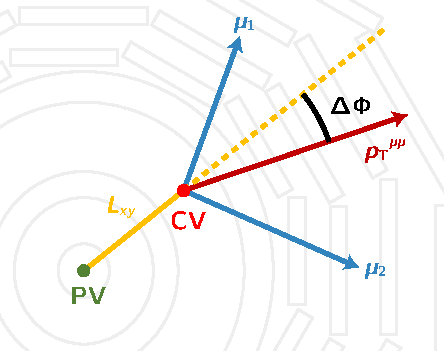
\includegraphics[width=.7\textwidth]{figures/displaced/LxyDef.pdf}
  \caption{Definitions}
  \label{fig:dd:LxyDef}
\end{figure}

\section{Event and Object Selection}
The general strategy for selecting reconstructed events and objects consistent with displaced dimuons is as follows.
\begin{enumerate}
  \item \textbf{DSA muon preselection}. Begin with DSA muons as seeds for searching for displaced dimuons and apply a set of quality criteria to select muons that are reasonably well reconstructed.
  \item \textbf{HLT-RECO matching}. Keep only events matching the HLT decision at the offline reconstructed level.
  \item \textbf{\DSAToPAT muon replacement}. Attempt to associate DSA muons with global or arbitrated tracker muons (referred to as PAT muons, named after the Physics Analysis Tools in the CMS software that processes them), and if they can be, replace the DSA muons with the associated PAT muons. This analysis focuses on the DSA muons that were not associated with PAT muons, so this step essentially rejects DSA muons that are consistent with muons reconstructed using both the tracker and the muon system.
  \item \textbf{DSA muon identification}. Apply additional selections to remaining DSA muons that identify DSA muons in signal-like events and ensure they are of good quality.
  \item \textbf{Dimuon formation from common vertex fit}. Form dimuons by fitting two DSA muon tracks to a common vertex.
  \item \textbf{Pairing criteria}. Select the 1--2 dimuons most likely to be signal dimuons according to a set of muon pairing criteria.
  \item \textbf{Dimuon identification}. Apply additional selections to dimuons that identify dimuons in signal-like events and ensure they are of good quality.
  \item \textbf{Dimuon signal selection}. Apply additional selections to dimuons that require the dimuon be displaced from the beamspot and have a form consistent with the signal hypothesis that the dimuon originates from the decay of a long-lived particle into two oppositely-charged muons.
  \item \textbf{Cosmic ray muon suppression}. Apply additional requirements to suppress background events from cosmic ray muons.
\end{enumerate}

\subsection{Event and Object Preselection}
\subsubsection{DSA Muon Quality Criteria}
\label{sec:dd:DSAQuality}
Event and object preselection begins with DSA muons.
The HLT path described in \Sec~\ref{sec:dd:trigger} reconstructs muons at \Ltwo using a procedure similar to that used to reconstruct muons as refitted standalone (RSA) muons at the offline reconstructed level.
However, as discussed in the previous section, DSA muons were chosen as the starting point over RSA muons for their improved \pT resolution and higher reconstruction efficiency.

The following quality criteria ensure that the DSA muons have acceptable \pT resolution and charge assignment, requiring that DSA muons
\begin{itemize}
  \item are reconstructed with hits in at least two muon stations, \ie $$N(\text{CSC stations}) + N(\text{DT stations}) > 1$$
  \item are reconstructed with at least 13 hits in the muon stations, \ie $$N(\text{CSC hits}) + N(\text{DT hits}) > 12$$
  \item have a fractional \pT error of less than 100\%, \ie $$\pTErr/\pT < 1$$
\end{itemize}

$$\text{PLOT OF PT RES AND CHARGE ASSIGNMENT FOR SIGNAL}$$

\subsubsection{HLT-RECO Matching}
Next, only events in which the HLT decision is matched using the preselected DSA muons are kept, in a procedure referred to as HLT-RECO matching.
This ensures that the quickly-reconstructed, coarser-resolution muons reconstructed by the trigger system have counterparts among muons reconstructed offline using the higher-precision data of the full event.
For the purposes of HLT-RECO matching only, DSA muons are required to pass loose \pT and $\eta$ requirements: $\pT > 10\GeV$ and $|\eta| < 2.0$.
These DSA muons are referred to as DSA muons for trigger matching.
Let \deltaR refer to the angular proximity in $\eta$-$\phi$ space between two three-vectors, defined as
\begin{equation}
  \Delta R = \sqrt{\Delta\eta^2 + \Delta\phi^2}
  \label{eq:dd:deltaR}
\end{equation}
Then HLT-RECO matching requires that a pair of distinct DSA muons for trigger matching lie within cones of $\deltaR < 0.4$ around each muon among pairs of muons reconstructed at \Ltwo passing the trigger (HLT muons).

The \pT, $\eta$, and \deltaR requirements were all chosen to heuristically optimize the tradeoff between efficiency and purity, matching as many events as possible while keeping the frequency of accidental matches to poor quality muons low.

$$\text{PLOT OF HLT MATCHING EFFICIENCY WRT TRIGGERED EVENTS IN SIGNAL}$$

The HLT-RECO matching requirement ensures, at the event level, that the trigger decision is confirmed using objects reconstructed offline.
The subsequent object selection, however, does not require that selected dimuons be formed from pairs of triggering HLT muons.
This allows the analysis to be sensitive to 4$\mu$ final states, in which two of the four muons passed the trigger, but all four muons are signal muons.

\subsection{\DSAToPAT Muon Replacement}
The position and momentum resolution of muons reconstructed using only the muon system is poorer compared to that of muons reconstructed using both the tracker and the muon system.
Beginning with DSA muons is essential to identify potential displaced muon events, but associating DSA muons to muons reconstructed using the tracker is critical to benefit from the improved resolution of the tracker.
Reconstructing muons with greater precision improves not only potential signal discrimination, but also background rejection.
Thus, a procedure was developed to associate DSA muons to muons reconstructed using the tracker.
Ensuring this procedure is both highly efficient (\ie muons that should be associated, are) and highly pure (\ie muons that should not be associated, are not) requires some care.
This section describes the details of the association procedure.

\subsubsection{PAT Muons and Matching Criteria}
Offline reconstructed muons having either of the following properties are considered:
\begin{itemize}
  \item \textbf{Global muons}. Global muons are muons reconstructed using a global refit of a tracker track and a standalone muon track.
  \item \textbf{Arbitrated tracker muons}. Tracker muons are muons reconstructed using a tracker track associated to hits in the muon system. The subset of tracker muons arbitrated such that no two tracker muons share muon segments are referred to as arbitrated tracker muons.
\end{itemize}
The muons considered in this analysis that are reconstructed offline using both the tracker and the muon system are referred to as PAT muons, PAT being an abbreviation for Physics Analysis Tools, a toolkit that is part of the CMS software and which is used to process event and object reconstruction.
A PAT muon may be both a global muon and an arbitrated tracker muon, and good quality PAT muons are indeed often both.

Candidate PAT muons are associated to DSA muons when they satisfy one of two matching criteria, which are applied in different contexts in a procedure described below. The two matching criteria are
\begin{itemize}
  \item \textbf{Segment-matched}: A PAT muon is segment-matched to a DSA muon if the PAT muon shares all of its muon system segments with all of the muon system segments used to reconstruct the DSA muon. PAT muon segments and DSA muon segments are compared coordinate by coordinate for equality and are considered the same if their coordinates match.
  \item \textbf{Proximity-matched}: A PAT muon is proximity-matched to a DSA muon if the \deltaR between
    \begin{itemize}
      \item the position vector of the innermost hit of the DSA muon and
      \item the momentum vector of the PAT muon helically extrapolated (in the magnetic field) to the point of closest approach to the innermost hit of the DSA muon
    \end{itemize}
    is less than 0.4, with tighter requirements applied in the procedure described below.
\end{itemize}

The proximity match is defined as it is above because DSA muons are sometimes reconstructed with an incorrect $\eta$ coordinate, and would not pass a more standard angular proximity match between the momentum directions of the DSA and PAT muons.
The helical extrapolation and comparison between the position and momentum improved the efficiency of the proximity match.

\subsubsection{\DSAToPAT Association Procedure}
The general procedure is as follows: given a DSA muon, take segment-matched PAT muons as the match, using additional quality criteria (requiring that muons be global and that they be reconstructed from hits in at least 7 tracker layers) and/or the PAT muon with the smallest proximity-match \deltaR (as defined above) to disambiguate among multiple segment-matched PAT muons.
If no PAT muons segment-matched the DSA muon, the smallest-\deltaR proximity-matched PAT muon is taken as the match if its proximity-match \deltaR is sufficiently small: the threshold is 0.1 if the proximity-matched PAT muon is global only, and 0.15 if the proximity-matched PAT muon is arbitrated tracker (whether or not it is global).
The full technical details of the procedure are depicted in \Fig~\ref{fig:dd:RepDiagram}.

\begin{figure}[p]
  \centering
  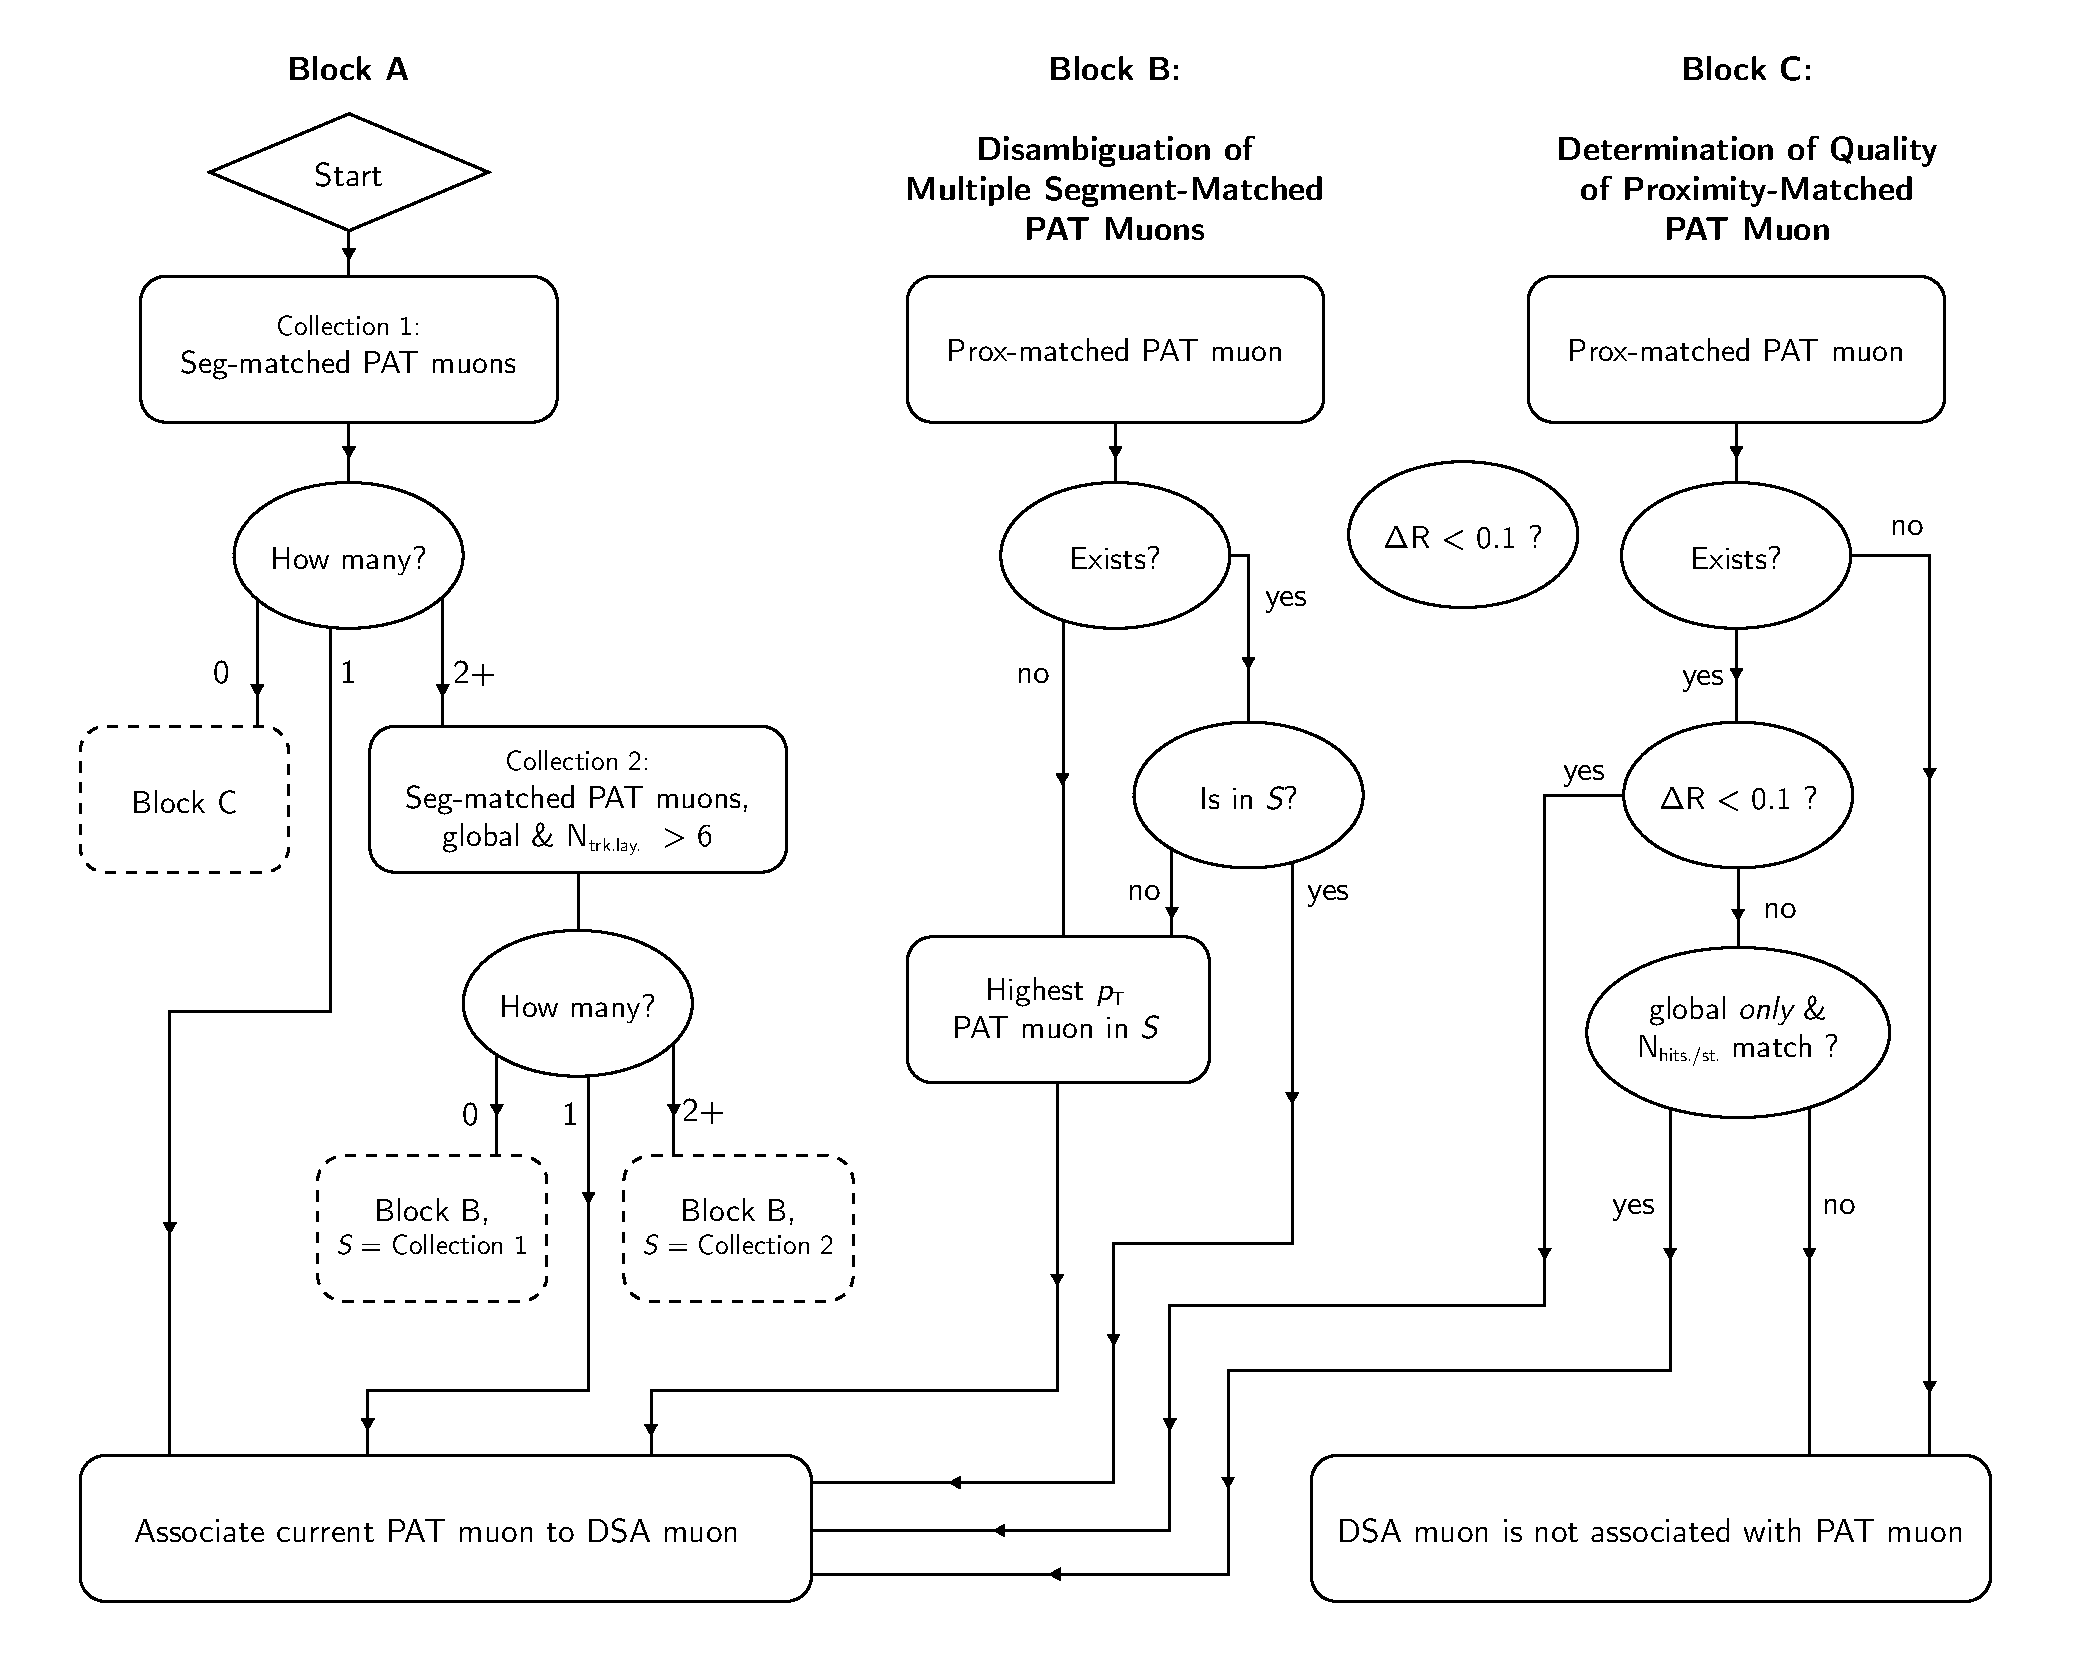
\includegraphics[width=\textwidth]{figures/displaced/ReplacementDiagram.pdf}
  \caption{Flowchart depicting the technical details of the \DSAToPAT replacement procedure. The procedure begins by considering segment-matched PAT muons. If there are multiple segment-matched PAT muons, then some temporary quality cuts are applied: the requirements that the muon be global and that it be reconstructed from at least 7 tracker layers (abbreviated $N_\text{trk. lay.}$). When there are multiple segment matches, the PAT muon that has the smallest proximity-match \deltaR is used to disambiguate between them, if possible. If there are no segment matches, then the proximity-matched PAT muon is taken as the match if its proximity \deltaR is sufficiently small, depending on whether the proximity-matched PAT muon is a tracker muon or only a global muon.}
  \label{fig:dd:RepDiagram}
\end{figure}

This procedure prioritizes segment-matched PAT muons over proximity-matched PAT muons.
Several combinations of criteria were used to determine the quality selection used to disambiguate segment-matched PAT muons; the combination used here (global and number of tracker layers) was found to be optimal in terms of increasing the efficiency to match to the correct PAT muon.
The fallback to the use of the highest \pT PAT muon among a collection of segment-matched PAT muons in the case that a proximity-match PAT muons does not exist or is not among the segment-matched PAT muons is only for logical consistency and is never a situation that actually occurs in practice.

The \deltaR thresholds in the case that there were no segment-matched PAT muons were chosen heuristically to increase the matching efficiency while keeping the rate of false, accidental matches low.
At the time of this writing, this analysis does not access the muon system segments used to reconstruct the standalone muons used to form global muons, and so a PAT muon that is global only cannot be segment-matched to a DSA muon.
This is an oversight that nonetheless has little practical effect on the efficiency to correctly associate DSA muons to PAT muons in this analysis.
For the small fraction of PAT muons that are global only and should be associated with a DSA muon, the proximity-matched PAT muon is often the correct choice, and so the \deltaR threshold for global-only PAT muons was set at 0.1.
The association procedure is also designed to be liberal: if a DSA muon can be reasonably associated with a PAT muon, it should be, even at the cost of a few accidental matches.
Therefore, in the case of no segment-matched PAT muons and a proximity-matched PAT muon that is a tracker muon, the procedure associates to the DSA muon the proximity-matched PAT muon if its proximity \deltaR is less than 0.15 as a final compromise between efficiency and purity.

As mentioned previously, the analysis presented in this thesis focuses only on the DSA muons that were not associated to PAT muons.
To this end, DSA muons are replaced with any associated PAT muons, and so the association step effectively functions as a rejection of DSA muons that can be associated to PAT muons.
The effects of this is that this analysis, using DSA muons, does not benefit from the improved resolution of PAT muons, benefits tremendously from the superior background rejection, and is the analysis sensitive to the longest lifetimes, with long-lived particles decaying in the outer region of the tracker and outside the tracker through the muon system.

$$\text{PLOT OF EFFECTS OF PAT REPLACEMENT ON SIGNAL AND ON MC BACKGROUND}$$

\subsection{DSA Muon Object Selection}
After the \DSAToPAT replacement step explained in the previous section, the analysis considers DSA muons not associated to any PAT muons.
As DSA muons are not used by many CMS analyses, a standard set of selections to identify DSA muons does not exist.
In order to further select high-quality DSA muons as well as discriminate signal-like events from background-like events, the following requirements, along with the DSA muon preselection cuts explained in \Sec~\ref{sec:dd:DSAQuality}, serve as the DSA muon identification selection.
DSA muons are required to have
\begin{itemize}
  \item muon $\pT$ of at least 10\GeV, \ie $$\pT > 10\GeV$$
  \item \normchisq of the muon track fit of at most 4, \ie $$\chisq_\text{track}/\text{dof} < 4$$
  \item at least 19 hits in the DTs for muons reconstructed only in the barrel, \ie $$N(\text{CSC hits}) = 0 \implies N(\text{DT hits}) > 18$$
\end{itemize}

The \pT cut suppresses background events which often have poor quality muons with low \pT, including background events arising from QCD processes.
The track \normchisq cut ensures that the muons are reasonably well reconstructed.
The $N(\text{DT hits})$ cut discriminates signal events from background events.

\subsection{Dimuon Formation from Common Vertex Fit}
A decay of a long-lived particle to two muons is detected as a pair of muons originating from a common vertex, so at this stage, pairs of reconstructed muons are investigated together for consistency with originating from a common vertex and from the decay of a massive, long-lived particle.
A pair of DSA muon tracks fit to a common vertex, along with the four-momentum sum of the two muons, is referred to as a dimuon.
All $n(n-1)/2$ possible pairs of distinct DSA muons among $n$ selected DSA muons are initially considered when forming dimuons.
This set of pairs is immediately filtered by requiring that the distance of closest approach (DCA) of the two DSA tracks helically extrapolated in the magnetic field is less than 50\unit{cm}:
$$\text{DCA} < 50\unit{cm}$$
This is a loose requirement ensuring that the common vertex fit is not performed on a pair of tracks that never come close to approaching each other.

\subsubsection{Vertex Fitting}
\label{sec:dd:vertexfitting}
The common vertex fit is performed by an implementation of the Kalman filter algorithm in the CMS software, called the \Code{KalmanVertexFitter}.
The implementation in the CMS software version used in this analysis restricts the range of the location of the fitted vertex to approximately within the boundary of the silicon tracker.
In this analysis, this restricted range is extended to the beginning of the muon system so as to efficiently reconstruct a common vertex for particles decaying outside the tracker.

The technical changes to the CMS software are documented here.
The following changes were made to \Code{RecoVertex/VertexTools/src/SequentialVertexFitter.cc}:
\begin{itemize}
  \item \Code{TrackerBoundsRadius} was changed from 112 to 500
  \item \Code{TrackerBoundsHalfLength} was changed from 273.5 to 1000
\end{itemize}

Only after a common vertex fit can the notions of dimuon quantities such as transverse decay length be defined.
As the existence of a common vertex fit is necessary to further study dimuon properties and consistency, the common vertex fit is required to converge.
The common vertex fit modifies the input tracks so as to be consistent with originating from a common vertex; these tracks are referred to as ``refitted'', and any of the muon properties (\pT, direction, \etc) may be different in the refitted version of the track than in the original version.
For many purposes, the refitted tracks are preferable because they represent a reconstruction performed with more information.
However, the vertex fitter fails or produces nonsensical results in a few situations.
A few of the features of the fitter are documented here.

The vertex fit does not always converge for an arbitrary pair of tracks.
FIGURE is a graph of the efficiency for the common vertex fit to converge, with respect to signal events passing the trigger in which both generated muons were reconstructed as DSA muons (where the matching between generated and reconstructed muons was performed using a \deltaR proximity between the momentum directions), as a function of the generated \Lxy.
$$\text{PLOT OF VERTEX FIT EFFICIENCY}$$
Convergence of the vertex fit is highly efficient when fitting two DSA muon tracks that are matched to generated signal muons produced from long-lived particle decaying in the detector up to transverse displacements of 330\unit{cm}.
Beyond 330\unit{cm}, the efficiency for the common vertex fit to converge drops dramatically.
Additionally, for those events beyond 330\unit{cm} that do converge, the \pT resolution of the refitted tracks are poorer, as seen in FIGURE.
$$\text{PLOT OF PT RESOLUTION LESS AND GREATER THAN 330 CM}$$
Finally, many of these events also retain an internal \Lxy uncertainty (\LxyErr) of a default value of 100\cm.
Such events would have a small \Lxy significance (3 or less) and would not pass an analysis selection.
This type of common vertex fit failure would result in the loss of these events, even though the fit converged.

As in the Run~1 analyses, the trigger efficiency at such large \Lxy values is quite small.
Therefore, further study of these events and attempts to rescue them from the behavior of the vertex fitter are of low priority for this analysis, and the underlying causes for this behavior remain a curiosity.

\subsection{Pairing Criteria}
\label{sec:dd:pc}
Since the efficiency to fit a common vertex to an arbitrary pair of DSA muons is high, considering all possible pairs of DSA muons results in many dimuons formed from DSA muons that are not related in any way, so it is important to develop criteria that choose the correct reconstructed dimuons, consistent with signal.
Selections on individual dimuons (such as requiring the \vchisq to be small) impose some quality constraints that are useful for selecting such dimuons, but any set of criteria that determines which pairs of muons form the correct dimuons must consider the event as a whole.
Choosing such a set of pairing criteria is particularly subtle in, for example, decays of two long-lived particles into a final state with 4 muons.
The 4 muons can be nominally paired into 6 overlapping dimuons, which can be partitioned into three distinct sets of 2 dimuons with no shared muons; the criteria must choose between them.
This situation is made more complex when, among other things,
\begin{itemize}
  \item one or more muons are not reconstructed
  \item duplicate muons are reconstructed from partial sets of hits
  \item muons are not all reconstructed with the correct charge
  \item pairs of muons are highly collimated and distinguishing them is difficult
  \item vertex fits of muons originating from different LLP decays yields a good \vchisq
\end{itemize}
\Fig~\ref{fig:dd:pc} is a diagram illustrating the application of the pairing criteria to the set of all possible dimuons in the case of four selected muons.

\begin{figure}[htpb]
  \centering
  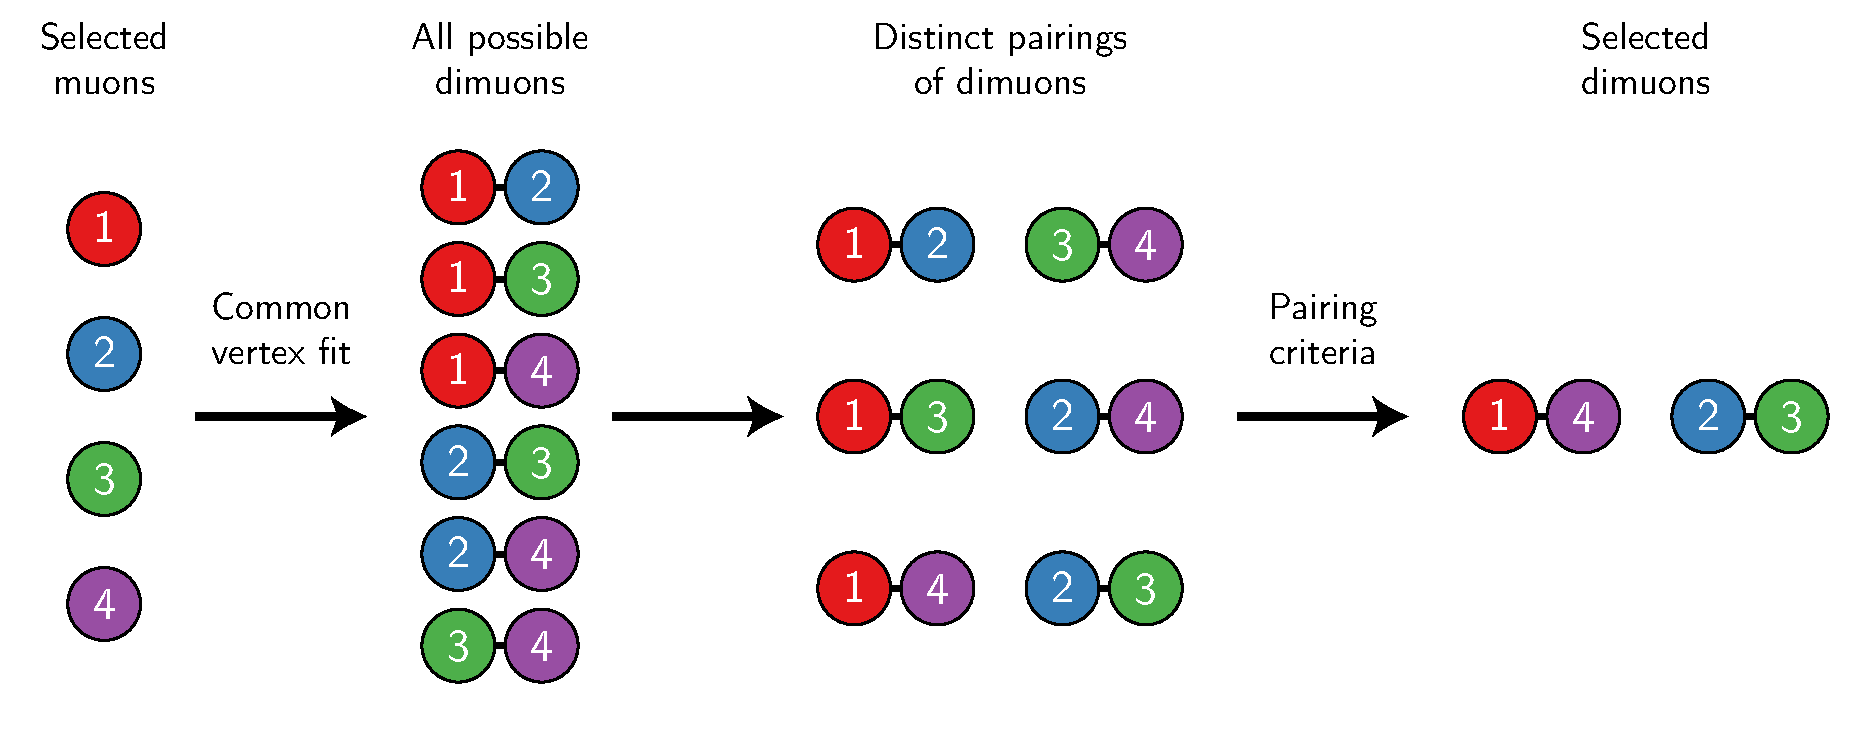
\includegraphics[width=\textwidth]{figures/displaced/PairingCriteriaDiagram.pdf}
  \caption{Diagram illustrating the application of pairing criteria to dimuons in the case of four selected muons. Four muons may be paired into six dimuons whose constituent muons overlap. These six dimuons may be partitioned into three distinct pairings of dimuons, in which no muons are shared between dimuons. Pairing criteria select the correct pair of dimuons consistent with a four muon signal event.}
  \label{fig:dd:pc}
\end{figure}

In developing this set of pairing criteria, several combinations of metrics were considered.
\begin{itemize}
  \item Dimuon(s) formed from the highest \pT muons in the event
  \item Dimuon(s) with the least \vchisq in the event
  \item Dimuon(s) formed from muons with charges of opposite sign
  \item Pairs of dimuons with the least sum of \vchisq
  \item Pairs of dimuons with the least difference in reconstructed dimuon mass
\end{itemize}

Potential pairing criteria were studied and optimized on both the 2$\mu$ and 4$\mu$ signal samples.
Choosing the highest \pT muons in the event is highly correlated with choosing the signal muons, a fact that is robust across all signal sample parameters covering a wide range of long-lived particle lifetimes and muon \pT spectra.
Requiring that dimuons be formed from muons of opposite charge provides only modest efficiency gains with respect to choosing the signal dimuons, and is undesirable at this stage as it introduces dependence on a specific type of signal model.
In events with less than four muons, a simple ranking of all possible dimuons by \vchisq yielded the highest efficiency.
The combinatorial space is far richer in events with four or more muons.
For long-lived particles decaying outside the tracker leading to events with at least 4 muons, the criterion yielding the highest efficiency to select signal dimuons is to choose the pair of dimuons whose \vchisq sum is the smallest, among all distinct pairs of dimuons that can be formed from the 4 highest \pT muons in the event. 
An alternative criterion to the least sum of \vchisq is the least difference in reconstructed dimuon mass.
Due to the limited mass resolution of DSA muons, this criterion was found to be less efficient overall than the least sum of \vchisq, except in events with a generated transverse decay length of less than 30\unit{cm}, a region where this DSA muon-based analysis has zero sensitivity.
Applying the pairing critera to an event with any number of dimuons formed from any number of muons results in 2 or fewer selected dimuons for the event.
The full technical details of this procedure are depicted in \Fig~\ref{fig:dd:pca}.

\begin{figure}[htpb]
  \centering
  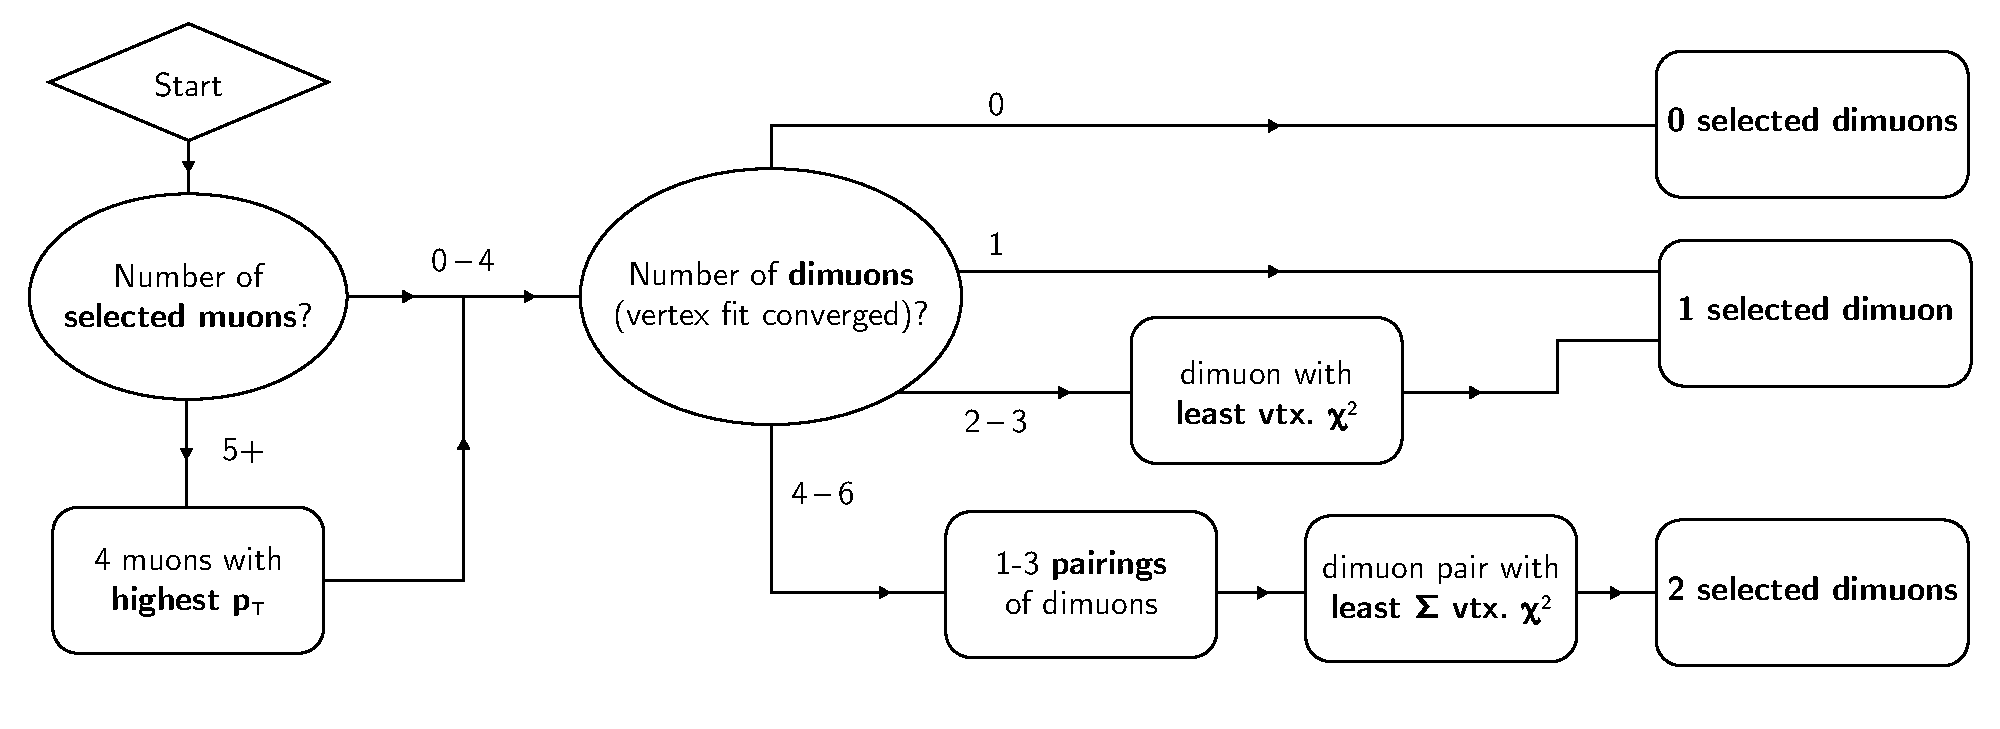
\includegraphics[width=\textwidth]{figures/displaced/PairingCriteriaAlgorithm.pdf}
  \caption{Flowchart depicting the technical details of the pairing criteria procedure. Up to 4 DSA muons are selected, ranked by \pT. With the DCA and vertex fit convergence requirements, these muons can be formed into up to 6 dimuons (0 for 0 or 1 muon, up to 1 for 2 muons, up to 3 for 3 muons, and up to 6 for 4 muons). The pairing criteria choose up to 2 dimuons among the possible dimuons.}
  \label{fig:dd:pca}
\end{figure}


$$\text{PLOT OF PAIRING CRITERIA EFFICIENCY}$$

\subsection{Dimuon Object Selection}
In order to further select high-quality dimuons as well as suppress background events, the following requirements, along with the DCA requirement, the requirement of convergence of the common vertex fit, and the application of the pairing criteria explained in \Sec~\ref{sec:dd:pc}, serve as a dimuon identification selection.
Dimuons are required to have a
\begin{itemize}
  \item reconstructed dimuon mass of at least 10\GeV, \ie $M_{\mu\mu} > 10\GeV$
  \item $\chi^2$ of the common vertex fit of at most 20, \ie $\chi^2_\text{vertex} < 20$
\end{itemize}

The \vchisq cut ensures that the dimuon is formed from tracks that can be reasonably well associated to a common vertex.
The mass cut suppresses complex backgrounds arising from QCD processes and events with low \pT and collimated muons.

\subsection{Dimuon Signal Selection}
The following criteria select displaced dimuons, consistent with the signal hypothesis of two muons with charge of opposite sign originating from the decay of a long-lived particle produced promptly, near the beamspot, resulting in a dimuon vertex displaced from the beamspot.
Dimuons are required
\begin{itemize}
  \item to have an \Lxy significance of at least 5, \ie $\Lxy/\LxyErr > 5$
  \item to have a transverse collinearity angle of less than $\pi/2$, \ie $|\DeltaPhi| < \pi/2$
  \item to be formed from two DSA muons with electric charges of opposite sign
\end{itemize}

\subsection{Cosmic Muon Suppression}
As mentioned in \Sec~\ref{sec:dd:vertexfitting}, one result of the common vertex fit of two muons is a pair of refitted tracks.
After the common vertex fit, a population of selected dimuons with relatively small \vchisq values was observed in data, and not in simulation, with the following unusual properties:
\begin{itemize}
  \item Muon refitted momentum $\phi$ directions changed in value by approximately $\pi$
  \item Muon refitted \pT uncertainties were unusually small, \ie $\pTErr/\pT \sim 10^{-7}\text{--}10^{-5}$
\end{itemize}
The presence of these dimuons were found to correlate with
\begin{itemize}
  \item Muons with relatively large transverse impact parameters, \ie $d_0 \sim 200\text{--}1000\cm$, and
  \item Events with no \pp collision vertices, and/or
  \item Events with large numbers of DSA muons, \ie $N(\text{DSA}) \sim 15\text{--}20$
    \begin{itemize}
      \item And these large numbers of DSA muons are largely parallel, \ie $|\cos(\alpha)| \sim 1$
    \end{itemize}
\end{itemize}
Further investigation suggested that these events are consistent with showers of cosmic ray muons.
\Fig~\ref{fig:dd:shower} is an example display of an event in data consistent with a shower of cosmic ray muons in a \pp collision event, containing a large number of approximately parallel pairs of DSA muons in addition to two global muons (not selected) originating from the \pp collision.

\begin{figure}[htpb]
  \centering
  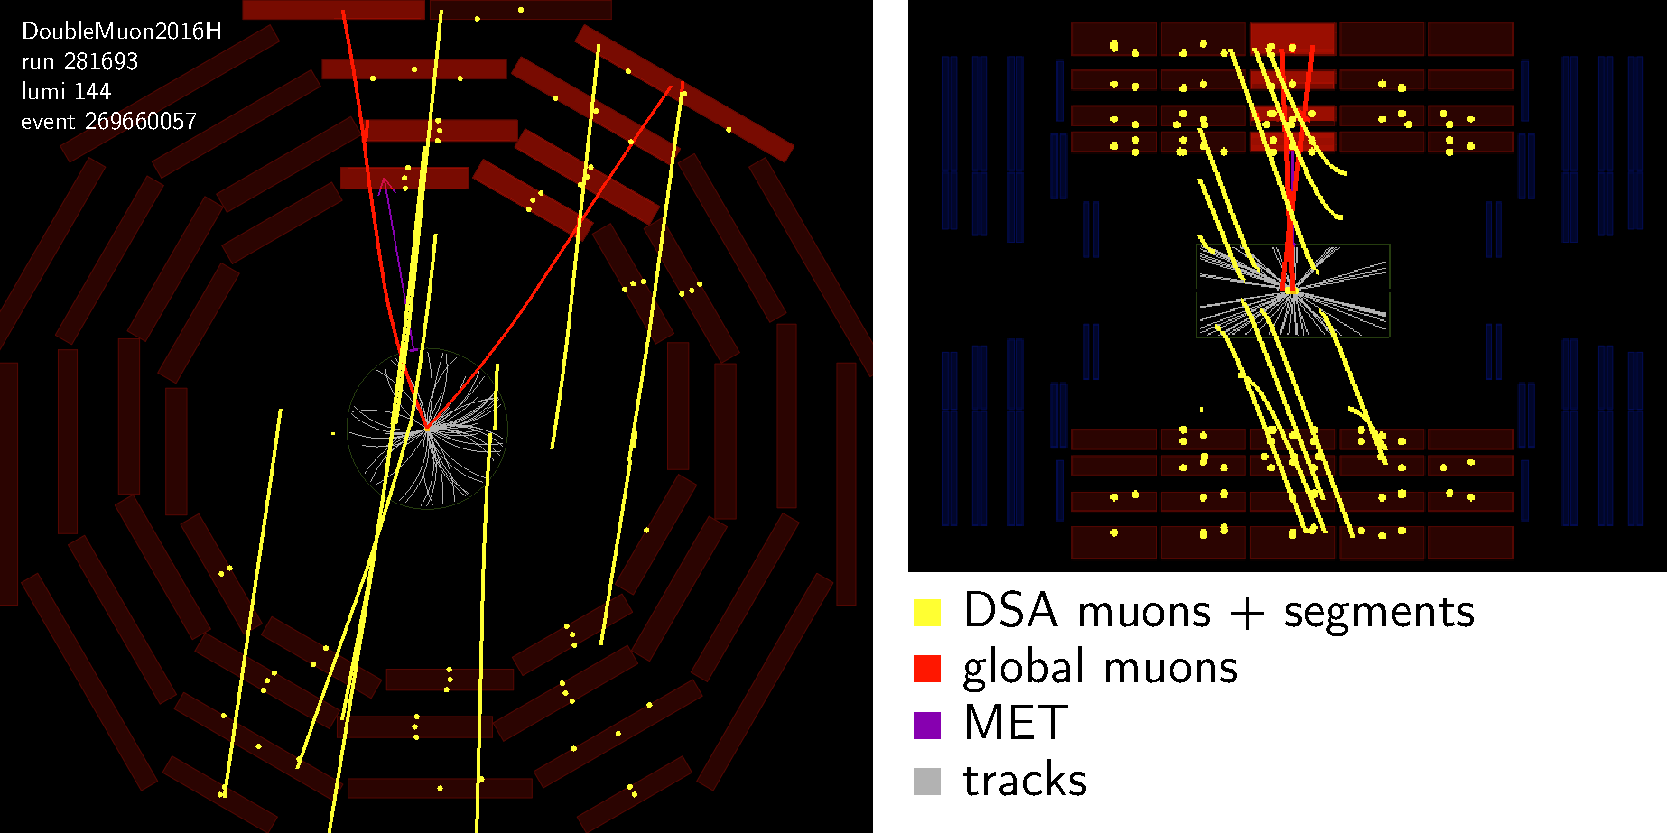
\includegraphics[width=\textwidth]{figures/displaced/ED_Cosmic.pdf}
  \caption{Display of an event in data consistent with a shower of cosmic ray muons in a \pp collision event. Two of the many approximately parallel DSA muons (yellow) reconstructed in this event formed a dimuon vertex with a good \vchisq and the event subsequently passed all our other selections. Requirements that events not contain too many parallel pairs of DSA muons and that the opening angle between the two muons not be too close to $\pi$ were found to be effective in suppressing such events.}
  \label{fig:dd:shower}
\end{figure}

A cosmic ray muon is often reconstructed as two back-to-back muons, one in the upper half of the detector and one in the lower half of the detector.
A reconstructed dimuon could also be formed from half a cosmic muon and a track from the \pp collision.
These dimuons are reconstructed as highly displaced, which is why the muons have such large $d_0$ values.
The common vertex fit was previously discussed to have anomalous behavior at large displacements, so the presence of the flip-by-$\pi$ and small \pT error anomalies when fitting to muons with large $d_0$ is perhaps not unexpected.
Such events are background events and so the analysis imposes a set of selections designed to suppress showers of cosmic muons.

Some of these events have no \pp collision vertices and contain only cosmic muons.
Events are therefore required to contain at least one well-identified vertex with position $(x, y, z)$ satisfying the following requirements:
\begin{itemize}
  \item At least 4 degrees of freedom when constructing the vertex
  \item $|z| < 24\mm$
  \item $\sqrt{x^2 + y^2} < 2\mm$
\end{itemize}
This set of requirements is referred to in CMS as the \Code{PrimaryVertexFilter}.

A typical strategy to suppress back-to-back cosmic muons is with a selection on $\cos(\alpha)$, and indeed the trigger has just such a cut, roughly equivalent to $\cos(\alpha) > -0.8$.
Following the trigger, our offline analysis selection also requires $\cos(\alpha) > -0.8$, on the opening angles both between the refitted muons and between the original (before the vertex fit) muons.

However, these two requirements alone are not sufficient to suppress all events consistent with cosmic muon showers.
As an additional measure to suppress cosmic muon showers, the analysis vetoes events with a large number of parallel pairs of DSA muons.
All possible pairs of DSA muons, with no common vertex fit, are considered, and the number of such pairs with $|\cos(\alpha)| > 0.99$, $N(\text{parallel pairs})$, are counted.
The analysis selection then requires that events contain no more than 5 such pairs.

In summary, the cosmic muon suppression selections are
\begin{itemize}
  \item Events pass the \Code{PrimaryVertexFilter}
  \item Events have $N(\text{parallel pairs}) < 6$
  \item Dimuons have original and refitted $\cos(\alpha) > -0.8$
\end{itemize}

\subsection{Summary of Event and Object Selection}
\Tab~\ref{tab:dd:fullsel} summarizes the full event and object selections discussed in this section.
\begin{table}
  \centering
  \begin{tabular}{llll} 
    \hline\hline
    \multicolumn{4}{c}{Event Selection} \\
    \hline
    primary vertex                    & \multicolumn{3}{l}{\Code{PrimaryVertexFilter} passed}       \\
    HLT-RECO matching                 & \multicolumn{3}{l}{HLT-RECO matching algorithm found match} \\
    number of parallel DSA muon pairs & $N$(parallel pairs)               & $>$ & 18                \\
    \hline
    & & \\

    \hline\hline
    \multicolumn{4}{c}{DSA Muon Selection} \\
    \hline
    replacement with PAT muons         & \multicolumn{3}{l}{DSA muons not associated to PAT muons} \\
    number of CSC and DT stations      & $N$(CSC+DT stations)             & $>$ & 1                \\
    number of CSC and DT hits          & $N$(CSC+DT hits)                 & $>$ & 12               \\
    number of DT hits for barrel muons & $N$(DT hits)                     & $>$ & 18               \\
    fractional \pT error               & $\pTErr/\pT$                     & $<$ & 1                \\
    transverse muon momentum           & \pT                              & $>$ & 10\GeV           \\
    normalized track \normchisq        & $\chisq_\text{track}/\text{dof}$ & $<$ & 4                \\
    \hline
    & & \\

    \hline\hline
    \multicolumn{4}{c}{Dimuon Selection} \\
    \hline
    distance of closest approach of muon & DCA                            & $<$ & 50\cm          \\
    common vertex fit                    & \multicolumn{3}{l}{common vertex fit converged}       \\
    pairing criteria                     & \multicolumn{3}{l}{best 1--2 ranked dimuons selected} \\
    dimuon mass                          & $M(\mu\mu)$                    & $>$ & 10\GeV         \\
    vertex \chisq                        & $\chisq_\text{vertex}$         & $<$ & 20             \\
    cosine of dimuon 3D opening angle    & $\cos(\alpha)$                 & $>$ & $-0.8$         \\
    \Lxy significance                    & $\Lxy/\LxyErr$                 & $>$ & 6              \\
    transverse collinearity angle        & $|\DeltaPhi|$                  & $<$ & $\pi/2$        \\
    opposite sign muons                  & \multicolumn{3}{l}{constituent muons are oppositely charged} \\
    \hline
  \end{tabular}
  \caption{Summary of full selection, organized into event, muon, and dimuon requirements.}
  \label{tab:dd:fullsel}
\end{table}

\clearpage
\subsection{Extra}

For each DSA muon:
\begin{enumerate}
  \item The set of segment-matched PAT muons among the set $P$ of all PAT muons is referred to as the set $P_\text{seg-matched} \subseteq P$.
    \begin{enumerate}[a.]
      \item If there are zero PAT muons in $P_\text{seg-matched}$, proceed to Step 2 using the set $P$; otherwise,
      \item If there is only one PAT muon in $P_\text{seg-matched}$, take it as the match; otherwise,
      \item If there are two or more PAT muons in $P_\text{seg-matched}$, consider the subset of segment-matched PAT muons that are both
        \begin{itemize}
          \item Global muons, and
          \item Reconstructed from hits in at least 7 tracker layers
        \end{itemize}
        referred to as the set $P_\text{clean} \subseteq P_\text{seg-matched}$.
        \begin{enumerate}[i.]
          \item If there is only one such PAT muon in $P_\text{clean}$, take it as the match; otherwise,
          \item If there are two or more such PAT muons in $P_\text{clean}$, proceed to Step 2 using the set $P_\text{clean}$; otherwise,
          \item If there are zero such PAT muons in $P_\text{clean}$, proceed to Step 2 using the set $P_\text{seg-matched}$.
        \end{enumerate}
    \end{enumerate}
  \item The set of proximity-matched PAT muons, $P_\text{prox}$, either contains the PAT muon $\mu_\text{prox}$ with the smallest proximity \deltaR or is the empty set. Consider $P_\text{prox}$ alongside the set of PAT muons $X$ determined by Step 1.
    \begin{enumerate}[a.]
      \item If $X$ is $P_\text{seg-matched}$ or $P_\text{clean}$
        \begin{enumerate}[i.]
          \item If $P_\text{prox}$ is empty or $P_\text{prox} \not\subset X$, take the highest \pT PAT muon in $X$ as the match; otherwise,
          \item If $\mu_\text{prox} \in X$, take it as the match.
        \end{enumerate}
      \item If $X$ is $P$
        \begin{enumerate}[i.]
          \item If $P_\text{prox}$ is empty, no match was found, and the DSA muon is not associated to a PAT muon; otherwise,
          \item If $\mu_\text{prox}$ is only global and its proximity $\deltaR < 0.1$, take it as the match; otherwise,
          \item If $\mu_\text{prox}$ is only tracker or global and tracker and its its proximity $\deltaR < 0.15$, take it as the match.
          \item Otherwise, the DSA muon is not associated to a PAT muon.
        \end{enumerate}
    \end{enumerate}
\end{enumerate}

\begin{itemize}
  \item \textbf{0--1 muons}: No dimuons can be formed.
  \item    \textbf{2 muons}: Keep the one dimuon that can be formed.
  \item    \textbf{3 muons}: Keep the dimuon with the lowest \vchisq among the 3 dimuons that can be formed.
  \item   \textbf{4+ muons}: Keep the \emph{pair} of dimuons with the lowest sum of \vchisq among the 3 pairs of dimuons that can be formed from the 6 dimuons that can be formed from the 4 muons with the highest \pT.
\end{itemize}
